\chapter{Sensitivity of the SuperNEMO demonstrator to the $\zeronu$}
\label{ch:sensitivity}


In this chapter, we present the SuperNEMO sensitivity to the $\zeronu$ decay half-life, and the corresponding effective neutrino masses, for several isotopes.
The SuperNEMO final detector is expected to exclude $\zeronu$ half-lives up to $1.2\times 10^{26}$ y ($90\%$ CL) if $\zeronu$ decays through the mass mechanism, with a detector exposure of $500$ kg.y \cite{art:SuperNEMO2010}.
The sensitivity is given as a limit, in case we do not observe the expected signal.
In $2010$ began the demonstrator installation at the Laboratoire Souterrain de Modane.
With an exposure of $17.5$ y, the demonstrator could set a limit on the $\zeronu$ process of $5.35\times 10^{24}$ y ($90\%$ CL) \cite{CalvezThesis}.

This study aims to explore the impact on the sensitivity of the presence of a magnetic field, and will participate in the final decision on the installation of the coil.
In a context of investigating the demonstrator and final detector capabilities, different internal source contamination levels are explored.
The topology of interest is the two electrons topology, and we use the $2e$ energy sum to discriminate the signal from the background events.
Thanks to SuperNEMO tracking capabilities, topological informations are exploited to improve the SuperNEMO sensitivity.



\section{Signal and backgrounds considered}

A full simulation for the SuperNEMO demonstrator was perfomed, in order to determine the longest $\zeronu$ half-life that can be probed with SuperNEMO using the distribution of the sum of electron energies, in the case where the $\zeronu$ decay were not observed.
In the Tab.~\ref{tab:sensitivity_simulations} is summarised the expected number of signal and background events, both for the SuperNEMO demonstrator and final detector, and we present the amount of simulated Monte-Carlo events for each considered decay.

\subsubsection*{The $\zeronu$ signal}

In the following, the assumed underlying mechanism for the $\zeronu$ decay is the mass mechanism (MM), as it is the most natural and widespread mechanism.
The hypotetical $\zeronu$ signal would be detected as an excess of events in the region of interest, with respect to the predicted background contamination level.
The $10^{7}$ $\zeronu$ Monte-Carlo events are generated using the DECAY$0$ software~\cite{art:decay0}.
The simulations are normalised assuming a $\Tbeta = 6.0\,10^{24}$ y half-life [citation].

\subsubsection*{Internal backgrounds}

As described in Sec.~\ref{subsec:SNbkg_internal}, source foils contaminations by isotopes such as \Tl\ or \Bi\ constitute the principal internal backgrounds with the $\twonu$ decay.
These backgrounds are processed by the same detector simulation as the $\zeronu$ signal, using DECAY$0$.
Since internal backgrounds have very low efficiencies in the $2e$ topology, we simulated an important amount of Monte-Carlo events.
The target background activities were defined so that each background has a similar contribution to that of the $\twonu$ in the region of interest~\cite{internal:SNphysicsCase}.\\
The dominant two neutrino $\twonu$ background and the background due to foil contamination were normalised assuming a detector exposure of $500$ kg.y.

\subsubsection*{Tracking volume background}


\subsubsection*{External background}

All external backgrounds from outside the foil, apart from \Rn\ in the tracking volume, are expected to be negligible and were not simulated.

\begin{table}[h]
  \caption{Expected and simulated decays for different processes, both for the demonstrator ($17.5$ kg.y) and for the final detector ($500$ kg.y).
  \label{tab:sensitivity_simulations}}
  \centering
  \begin{tabular}{|c|cc|c|}
    \hline
    &\multicolumn{2}{c|}{Expected decays} & Simulated decays \\
    & Demonstrator & Final detector & \\
    \hline\hline
    $\zeronu$ ($\Tbeta = 6.0\,10^{24}$ y) & $1.5\,10^{1}$ & $2.7\,10^{7}$ & $1.0\,10^{7}$ \\
    $\twonu$ & $9.5\,10^{5}$ & $4.2\,10^{2}$ & $1.0\,10^{7}$ \\
    \Tl  & $5.5\,10^{3}$ & $1.6\,10^{5}$ & $1.0\,10^{7}$ \\
    \Bi  & $1.1\,10^{3}$ & $3.1\,10^{4}$ & $1.0\,10^{7}$ \\
    \Rn  & $1.8\,10^{5}$ & $7.2\,10^{6}$ & $1.0\,10^{7}$ \\
    \hline
 \end{tabular}
\end{table}

\begin{figure}[h]
  \centering
  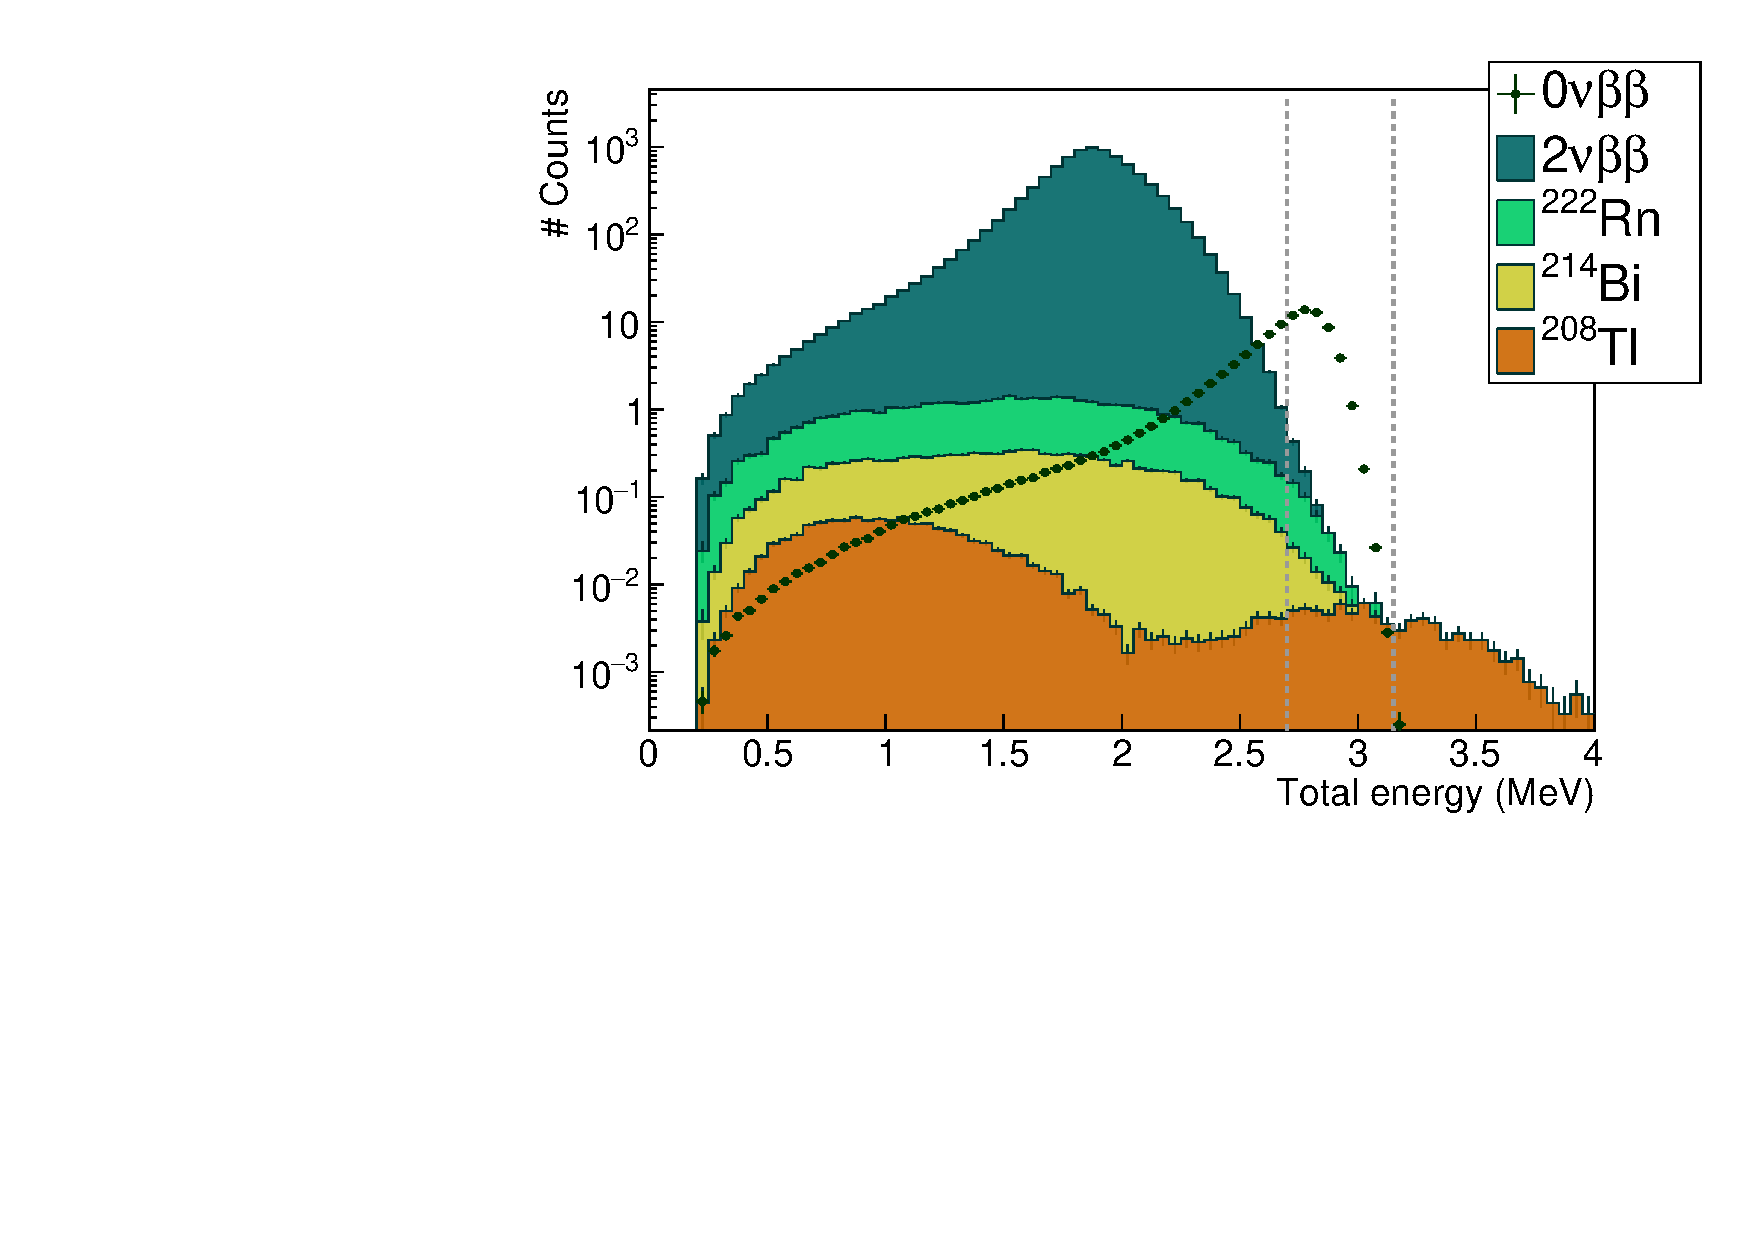
\includegraphics[width=1.1\textwidth]{Sensitivity/fig_sensitivity/energy_spectrum_with_B_82Se.pdf}
  \caption{
    \label{fig:sensitivity_energy_spectra}}
\end{figure}







Justifier bdf externe avec article nemo3 (plus diff roi et meilleure eff)
Activités bkg considérées à justifier, bkg interne: balek externe à justifier\\

Demies vies 2nu à jusifier


Se, Nd avec et sans champs\\
présentation du PID de Steven (peut être à bouger dans Tl selon développement du plan ou généralités)

Influence des quantités de contaminations sur la sensibilité

\section{Optimisation of event selection}
plot S/sqrt(B) en fonction E>Emin\\


Quel est le signal qu'on cherche\\
présentation des cuts\\
efficacité des cuts/ signal + bkg\\
cuts premier et second ordre
\section{Expected number of background events}
plot energy tot
plus dans région intéret


\section{Demonstrator sensitivity}
Résultats $B=0$, avec activités nominales, puis avec activités caca\\
Efficiency spretra\\
Energy spectra

\subsection{avec B}
Parler du champ non uniforme/attenuation
ROI optimization: avec variation coupure énergie\\

\subsection{sans B}
avec variation coupure énergie\\

\subsection{Champ mappé}


\section{HyperNEMO}
results for $500$kg.y exposure

\section{Other isotopes}
bam bam le Nd

distribution t1/2 avec différents échantillons de simus (17.5 kg.y)

\section{Conclusion}
Faut arrêter SN\\
Etude plus générale avec bkg externe+lab (reprendre chiffres NEMO3)
+ neutrons (cf NEMO3)
